\documentclass[a4paper,10pt]{article}
%\documentclass[a4paper,10pt]{scrartcl}
\usepackage{hyperref}
% \usepackage{caption}
\hypersetup{pdfborder={0 0 0}}
\usepackage[all]{hypcap}
\usepackage{default}
\usepackage{graphicx}
\usepackage{array}
\usepackage{amsmath}
\usepackage{listings}

\lstset{language=Python,% general command to set parameter(s)
basicstyle =\small\ttfamily,          % print whole listing small
showstringspaces=false,
commentstyle=\ttfamily}

\title{Backprop exercises}
\author{Olivia Guest}
\date{\today}

\begin{document}
\maketitle
\section{Running a perceptron on paper}
\begin{figure}[hb]
 \centering
 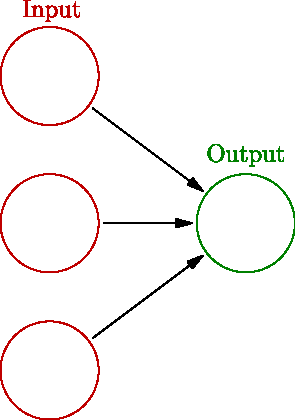
\includegraphics{../slides/fig/perceptron_empty.pdf}
 \caption{A perceptron that you can run on paper.}
 \label{fig:perceptron}
\end{figure}
Using the activation propagation \autoref{eq:propagate} as presented and applied in the handouts calculate the output of the perceptron in \autoref{fig:perceptron}:
\begin{equation}
\label{eq:propagate}
y = f\left(  \sum_{j=1}^N x_j \times w_{ji} \right)
\end{equation}

Firstly, because this is just a practice run to help you understand how activations propagate randomly, choose some values for the weights and inputs (simple small numbers will make the arithmetic easier). Then, using the three inputs and the three connection weights you just picked, calculate the value of the single output unit. If you wish to calculate the so-called post-synaptic activation for the output unit you can use an activation function. A simple version of this function, denoted by $f$, is to change the output unit's value to $1.0$ if the total of all inputs to it is above $0$, otherwise set it to $0$. In other words:
\begin{equation}
\label{eq:f}
  y = \left\{ 
  \begin{array}{l l}
    1 & \quad \text{if $ \sum_{j=1}^N x_j \times w_{ji} > 0$ }\\
    0 & \quad \text{otherwise}\\
  \end{array} \right.
\end{equation}


What does $f$ help the network do?


\section{Playing around with the network}
Now you will have a go playing around, but hopefully not breaking, the network depicted in \autoref{fig:perceptron_maths}. However, don't worry if you do break it, there is an infinite supply.

\begin{figure}[hb]
\centering
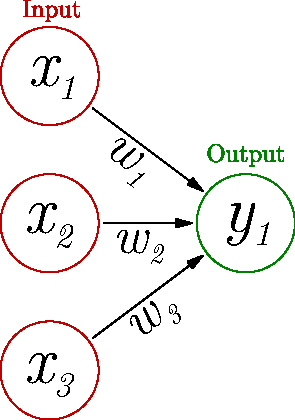
\includegraphics{../slides/fig/perceptron_maths.pdf}
\caption{A perceptron}
\label{fig:perceptron_maths}
\end{figure}

Have a look at the code that makes it learn. Open the file called \texttt{pyceptron.py} and go to the part that says \texttt{def Train(self):}. This function, as I probably already explained, does a bunch of things that essentially implement the two basic equations. The first equation is that for calculating the activation of the output unit(s): 
\begin{equation}
y_j = f \left( \sum_1^N w_i \times x_i \right)
\end{equation} 
where $y_j$ is the (output) unit whose state you want to calculate, $N$ is the number of units on the previous layer, $w_{i}$ is the weight on the connection between $i$ and $j$, and $f$ is a function that the unit applies. In the code you can write that in many ways, just like you can say the same or similar things in natural language in a number of different ways. I decided on this:
\begin{lstlisting}
for i in range(N+1): 
	y += x[i] * w[i]
	
y = f(y)
\end{lstlisting}
and hopefully you can guess what each variable is based on the equation. Find this snippet of code within the \texttt{Train} function. Using your own judgement, add some comments to explain what is going on, for example:
\begin{lstlisting}
              for i in range(N+1): 
              # loop through all the indices of input units
                      y += x[i] * w[i]
                      # sum the product of each input unit x[i]
                      # and weight w[i] and save it in output
                      # unit y
                      
              y = f(y)
              # calculate the post-synaptic value for y
\end{lstlisting}
Ask for help if something is not making sense straight away.
\\ \ 

Can you find where \texttt{f} is defined?
\\ \

The second, and equally important equation, you need is the one that trains the weights:
\begin{equation}
\Delta w_i = \eta  ( d_j - y_j ) \times x_{i}
\end{equation} 
where $d$ is what you want $y$ to be given $x$, and $\eta$ is the learning rate. In other words $d$ is the target, $y$ is as before the output unit (or units), and $x$ are the unit units. As before, there are a number of different ways to say this in Python. Hopefully, my choice is a clear translation:
\begin{lstlisting}
                   error = d[p][0] - y
                   
                   for i in range(N+1): 
                      w[i] += h * error * x[i]\end{lstlisting} 



Now that you have a slightly clearer idea (if not --- ask me or a demonstrator for clarification) of how the network works, have a go changing things to see what happens. Before you change anything though, try running the network to see what happens with the current settings.

\begin{enumerate}
 \item Can you figure out what it is learning based on the output it prints to screen?

 \item After how many iterations does it learn (i.e., have no error)?
\end{enumerate}

Now try the following:

\begin{enumerate}
 \item Change the number of training iterations as set in \texttt{Main()}. What happens?
 \item Change the value of the learning rate as set in \texttt{Main()}. What happens?
 \item What does \texttt{N.Run()} do? Try commenting it back in to see.
 \item \texttt{N.Run()} calls the function \texttt{def Run(self):} (below \texttt{Train}) --- can you tell now what it might do?
 \item Can you spot similarities (and differences) between \texttt{Run} and \texttt{Train}? Imagine if it was called something less informative than  \texttt{Run}, would you still be able to reverse-engineer it? Add comments to help you if you need to return to it.
 \item Change the \texttt{graphs} parameter in the initialisation of the network \texttt{N} to \texttt{True}. What happens?
 \item Is there something with respect to the actual running or training of the network that you do not understand? Try to use \texttt{print} to see what is going on in such a case.
\end{enumerate}


With respect to the graphs, they represent what the network knows about the inputs. Inputs that are classed as 1.0 (their target is 1.0) are represented with one colour and inputs in the other class are coloured with another. The line that moves around during training is a function of the weights and shows how the network is separating the data into two groups (i.e., $y$ is either 1.0 or 0.0). In other words, the graph depicts that training set as points in a two dimenstional space and the line depicts the weights. If the training set can be linearly separated, i.e., if the line can dissect the input patterns into two classes that reflect the targets then the network has represented the training set correctly.
\ \\ 
\ \\ 
What do the x and y axes represent in the graph? Compare the points' coordinates with the values of the input patterns.
\ \\ 
\ \\ 
Based on these graphs can you tell when the network has learned?
\ \\ 
\ \\
Is the concept of linear separation useful to keep? If you think so, keep the \texttt{graphs} set to \texttt{True} for the next section of coding.


\section{Teaching the network logic}
To explore some of the  very basic uses of neural networks, you will first attempt to teach the perceptron logical operators. Logical operators were touched on in the first part of the workshop, when we talked about \textbf{not}, \textbf{and}, \textbf{or}, etc., and applied them to truth values (i.e., true and false).

Even though logical operators might seem very abstract, saying things like ``true \textbf{and} true is true'' is just a formalised way of saying much more common expressions such as ``I agree \textbf{and} you agree, therefore we both agree''. Natural language is full of such logical operations, for example when we ask questions, e.g., ``do you want sugar \textbf{or} milk in your tea?'' is equivalent to ``sugar \textbf{or} milk'' in formal logic (recall this allows for both as well as either). Such formalisation is useful because it is an easy way to avoid ambiguity, thus helping us gain a clear understanding of what a network is telling us. 

\subsection{Not}

The first logical operator you will teach your perceptron is the \textbf{not} operation. This requires one input unit and one output unit because negation (a synonym for not) is applied to one variable (or in our case input unit) at a time. So when you give the network a 0 you want it to return a 1, and when you give the network a 1 you need a 0 on the output. That means our training patterns are 0 and 1, and our targets are 1 and 0, in that order. \autoref{tbl:not} represents our patterns and their required targets. 
%modify this section to say where in the code you need to edit stuff

\begin{table}[htb]
 \centering
 \begin{tabular}[t]{cc}
Input & Output\\ \hline
0 & 1\\
1 & 0
\end{tabular} \caption{Truth table for logical \textbf{not}.}
 \label{tbl:not}
\end{table}

Once you have made the required changes, run the network to see what happens and how long it takes to train. 

\ \\ Can the network learn \textbf{not}?    Yes / No           

\ \\ Is \textbf{not} linearly seperable? Yes / No
                                                     

\subsection{And}

Now let's teach it something a little more complex, the most basic form of logical \textbf{and} is that with two inputs (e.g., false \textbf{and} true is false) and it always has one output. Meaning that the network needs to learn the input-output mapping given in \autoref{tbl:and}. By looking at \autoref{tbl:and}, you might notice that now there are three units, two input units and the same number of output units as before. So you need to modify the network to have two input units, leaving the single output unit untouched. Thankfully, the code can figure out the number of input and output units required based on the patterns and targets you give it. This is because when I wrote the code I made no assumptions about the number of input units. I did however make a strong assumption that there is only a single output unit (i.e., the targets are always one value long), to keep the code a little simpler. 
% This is something I wrote myself, if you want to see how that is done feel free to play around with the , but do not get bogged down with understanding this  %modify this section to say where in the code you need to edit stuff
Once the patterns and targets are set, run the network like before and see what happens.

\ \\ Can the network learn \textbf{and}?    Yes / No                                             

\ \\ Is \textbf{and} linearly seperable? Yes / No

\begin{table}[ht]
 \centering
 \begin{tabular}[t]{ccc}
Input 1 & Input 2 & Output\\ \hline
0 & 0 & 0\\
0 & 1 & 0 \\
1 & 0 & 0 \\
1 & 1 & 1 \\

\end{tabular} \caption{Truth table for logical \textbf{and}.}
 \label{tbl:and}
\end{table}

\subsection{Or}

Now let's do the same for \textbf{or}. Logical \textbf{or} returns a 1, or true, if either input is on. In other words, it only returns 0 when neither are 1, as shown in \autoref{tbl:or}. Remember that at any point you can check what any logical operator does directly in the Python shell, e.g., by typing \texttt{False or True}, Python will say \texttt{True} (corresponding to the 3rd line of \autoref{tbl:or}).

\ \\ Can the network learn \textbf{or}?    Yes / No         

\ \\ Is \textbf{or} linearly seperable? Yes / No                                    

\begin{table}[ht]
 \centering
 \begin{tabular}[t]{ccc}
Input 1 & Input 2 & Output\\ \hline
0 & 0 & 0\\
0 & 1 & 1 \\
1 & 0 & 1 \\
1 & 1 & 1 \\

\end{tabular} \caption{Truth table for logical \textbf{or}.}
 \label{tbl:or}
\end{table}

\subsection{Could the network buy me fruit?}
 Instead of only learning the outcomes of logival operators the network can try to clasify some fruit based on two of their features, colour and taste, into ones I do and ones I do not want to eat. Can the network learn which of the fruit in \autoref{tbl:fruit} I like?
 



\begin{table}[ht]
 \centering
 \begin{tabular}[t]{cccc}
Name & Colour &  Taste & Does Olivia like it? \\ \hline
& Yellow-Red & Sour-Sweet & Yes-No \\ \hline
Loquat & 0.1 & 0.5 & 1.0 \\
Lemon & 0.0 &  0.0 & 0.0 \\
Apple & 1.0 &  0.8 & 0.0 \\
Strawberry & 1.0 &  0.9 & 1.0 \\
   
\end{tabular} \caption{Some fruit for the network to categorise.}
 \label{tbl:fruit}
\end{table}


\ \\ Can the network classify the fruit based on my personal preferences?    Yes / No   

\ \\ Is it an easy classification for the network to learn? Yes / No

\ \\ Does changing the learning rate help?    Yes / No   

\ \\ Does training for longer help?    Yes / No   




\subsection{Xor}
Things start to become interesting when you teach the network \textbf{xor}, also known as exclusive or. Like its namesake \textbf{or}, \textbf{xor} returns true when either one or the other inputs are true, \emph{but it does not} return true when both are true (compare \autoref{tbl:xor} with \autoref{tbl:or}).  


In Python one way of specifying \textbf{xor} is by using \texttt{(a and not b) or (b and not a)}. You do not need to know this to program the network, because the network figures out how to map inputs onto outputs itself, or at least tries to...

\begin{table}[ht]
 \centering
 \begin{tabular}[t]{ccc}
Input 1 & Input 2 & Output\\ \hline
0 & 0 & 0\\
0 & 1 & 1 \\
1 & 0 & 1 \\
1 & 1 & 0 \\

\end{tabular} \caption{Truth table for logical \textbf{xor}.}
 \label{tbl:xor}
\end{table}


\ \\ Can the network learn \textbf{xor}?    Yes / No   

\ \\ Is it an easy classification for the network to learn? Yes / No

\ \\ Does changing the learning rate help?    Yes / No   

\ \\ Does training for longer help?    Yes / No   

\ \\  Describe what is going on here.



\end{document}
